\chapter{Detekce příjmu karbohydrátů}

Pro detekci příjmu karbohydrátů jsem měl k dispozici anonymizovaná data ze senzoru CGMS. Data obsahují naměřené a zadané hodnoty:
\begin{itemize}
\setlength\itemsep{0em}
\item Glukóza v krvi (BG)
\item Intersticiální glukóza (IST)
\item Bazální množství inzulinu
\item Bolus inzulinu
\item Příjem karbohydrátů (CHO)
\item Fyzická aktivita
\item Kvalita spánku
\item Počet kroků
\item Srdeční tep
\item Vodivost kůže
\item Teplota kůže
\item Teplota okolí
\end{itemize}

Rozhodl jsem se vyzkoušet 3 metody:
\begin{itemize}
\setlength\itemsep{0em}
\item Lineární a kvadratická diskriminační analýza (kapitola \ref{ch:lda_qda})
\item Long short-term memory neuronová síť (kapitola \ref{ch:lstm})
\item Metoda thresholdů 1. derivace hodnot intersticiální glukózy \\(kapitola \ref{ch:threshold})
\end{itemize}

Programovací jazyk pro zpracování dat ze senzoru, návrh a vyhodnocení jednotlivých metod jsem zvolil Python. Python jsem zvolil pro jeho knihovny numpy, pandas a scipy pro zpracování a analýzu dat a matplotlib pro vykreslení dat. Přestože je Python interpretovaný jazyk a tudíž pomalý při zpracování velkého množství dat, tyto knihovny jsou implementovány v jazyce C a optimalizovány pro vysoký výkon. Doba zpracování dat je tak srovnatelná s jinými kompilovanými jazyky.

Implementace do SmartCGMS je v jazyce C++.

\newpage

\section{Příprava dat}

CGMS senzor posílá data ve formě signálů, které mají strukturu:
\begin{itemize}
\setlength\itemsep{0em}
\item Logical Clock
\item Device Time
\item Event Code
\item Signal
\item Info
\item Segment Id
\item Event Code Id
\item Device Id
\item Signal Id
\end{itemize}

Příklad signálů ze senzoru CGMS je v tabulce \ref{tab:cgms_data}

\begin{table}[H]
\caption{Signály ze CGMS}
\label{tab:cgms_data}
\centering
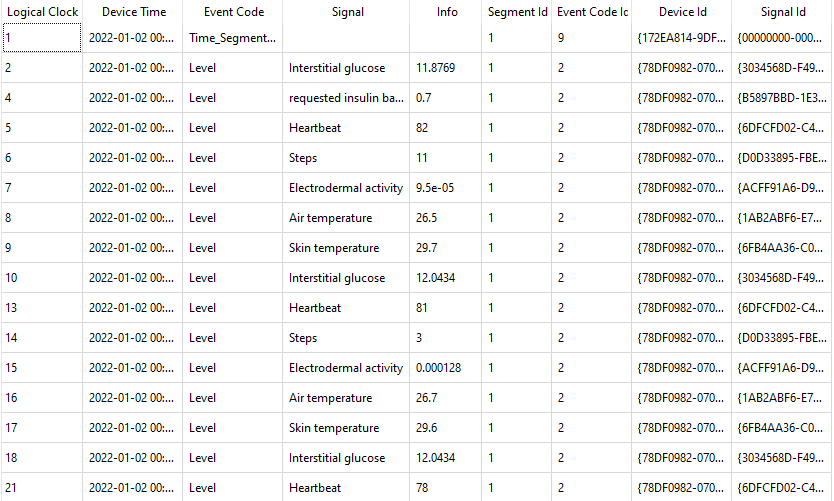
\includegraphics[width=1\textwidth]{img/cho/cgms_data.png}
\end{table}

Informaci pro následnou detekci v sobě nesou sloupce Device Time (čas měření), Signal (typ signálu) a Info (hodnota). Ty jsem extrahoval do dvourozměrné tabulky, kde řádky jsou čas měření a sloupce jednotlivé typy signálů.
Data interstciální glukózy jsem interpoloval Akima spline \citep{cho.akima}, z níž jsem získal chybějící hodnoty a derivace 1. 2. a 3 řádu. Pro vyhlazení hodnot intersticiální glukózy jsem použil Savitzky-Golay filtr \citep{cho.savgol} řádu 3 s velikostí okna 51. Jelikož různé typy signálu nejsou měřeny ve stejný okamžik, řádky jsem seskupil podle sloupce intersticiální glukózy, která je měřena v pětiminutových intervalech.

V grafech na obrázku \ref{fig:48h_dataset} jsou transformovaná data naměřená senzorem CGMS za 48 hodin. Na prvním grafu jsou hodnoty Intersticiální glukózy a její vyhlazení Savitzky-Golay filtrem. Druhý graf znázorňuje zadanou bazální dávku inzulinu, bolusy, příjem karbohydrátů a fyzickou aktivitu. Na posledním grafu jsou zbylé měřené hodnoty.

\begin{figure}[H]
\caption{Data ze CGMS}
\label{tab:48h_dataset}
\centering
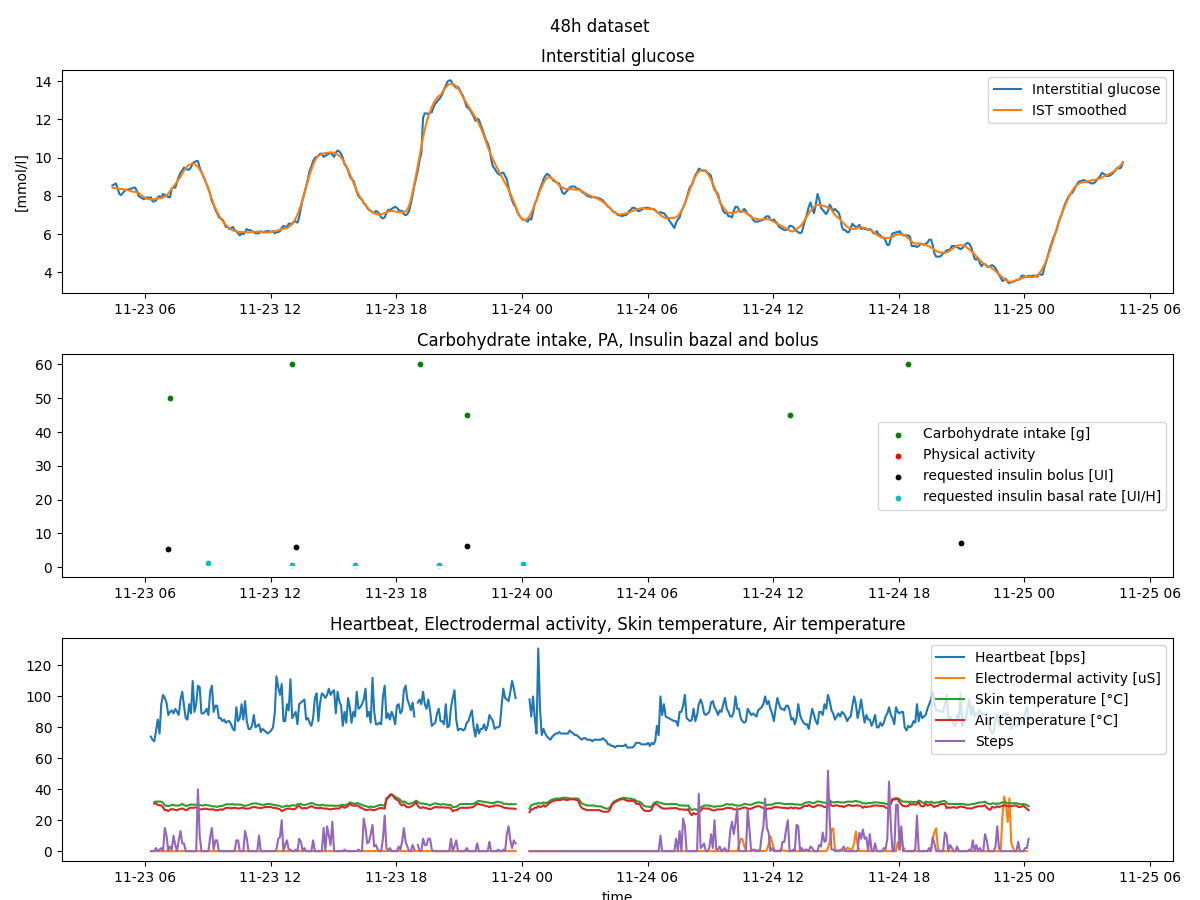
\includegraphics[width=1\textwidth]{img/cho/48h_dataset.png}
\end{figure}

Python script zpracování dat je v souboru load\_data.py.

\section{Lineární a kvadratická diskriminační analýza}
\label{ch:lda_qda}

Lineární diskriminační analýzu jsem se rozhodl implementovat vzhledem k vysoké úspešnosti a malému zpoždění, které dosáhli \citet{Analyza.LDA} v článku \textbf{Pattern Recognition Reveals Characteristic Postprandial Glucose Changes: Non-Individualized Meal Detection in Diabetes Mellitus Type 1} (kapitola \ref{ch:lda}).

Diskriminační analýza


\section{Long short-term memory}
\label{ch:lstm}


\section{Threshold 1. derivace IST}
\label{ch:threshold}
